%% LyX 2.2.3 created this file.  For more info, see http://www.lyx.org/.
%% Do not edit unless you really know what you are doing.
\documentclass[english,12pt]{article}
%\usepackage[LGR,T1]{fontenc}
\usepackage[utf8]{inputenc}
\usepackage{geometry}
\geometry{verbose,tmargin=2cm,bmargin=2cm,lmargin=2cm,rmargin=2cm}
\usepackage{array}
\usepackage{float}
\usepackage{booktabs}
\usepackage{textcomp}
\usepackage{multirow}
\usepackage{amsmath}
\usepackage{amsthm}
\usepackage{amssymb}
\usepackage{authblk}
\usepackage{sectsty}
\usepackage{hyperref}
\usepackage{graphicx}
\usepackage{blindtext}
\usepackage{caption}
\usepackage{subcaption}
\usepackage{lmodern}
\usepackage{xcolor}
\usepackage{multicol}
\usepackage{bm}
\usepackage{mathtools}

%%% DAG & SWIG Stuff
\usepackage{tikz}
\usetikzlibrary{arrows,automata}
\tikzset{
	semi/.style={
		semicircle,
		draw,
		minimum size=2em
	}
}

\usetikzlibrary{shapes, snakes, graphs, shapes.geometric, positioning}


\sectionfont{\fontsize{14}{13}\selectfont}
\subsectionfont{\fontsize{12}{12}\selectfont}



\allowdisplaybreaks

\makeatletter

%%%%%%%%%%%%%%%%%%%%%%%%%%%%%% LyX specific LaTeX commands.
\DeclareRobustCommand{\greektext}{%
  \fontencoding{LGR}\selectfont\def\encodingdefault{LGR}}
\DeclareRobustCommand{\textgreek}[1]{\leavevmode{\greektext #1}}
\ProvideTextCommand{\~}{LGR}[1]{\char126#1}

%% Because html converters don't know tabularnewline
\providecommand{\tabularnewline}{\\}

%%%%%%%%%%%%%%%%%%%%%%%%%%%%%% Textclass specific LaTeX commands.
\theoremstyle{plain}
\newtheorem{thm}{\protect\theoremname}

%%%%%%%%%%%%%%%%%%%%%%%%%%%%%% User specified LaTeX commands.
\usepackage{amsmath}
% \usepackage[table]{xcolor}% http://ctan.org/pkg/xcolor


\makeatother

\usepackage{babel}
\providecommand{\theoremname}{Theorem}

% Define independence command
\newcommand\independent{\protect\mathpalette{\protect\independenT}{\perp}}
\def\independenT#1#2{\mathrel{\rlap{$#1#2$}\mkern2mu{#1#2}}}



%%%% April 2024 update - new color palette %%%%%
%%%%%%%%%%%%%%%%%%%%%%%%%%%%%%%%%%%%%%%%%%%%%%%%
\definecolor{halenavy}{HTML}{4F6469}
\definecolor{steel}{HTML}{779D9D}
\definecolor{sky}{HTML}{B6D9D3}
\definecolor{grove}{HTML}{EEF3DA}
% please use orangepeel and grapefruit sparingly
\definecolor{orangepeel}{HTML}{FEC36B}
\definecolor{grapefruit}{HTML}{FE7C76}

% Secondary colors - see branding book for guidance on using secondary colors
\definecolor{pine}{HTML}{70A586}
\definecolor{berry}{HTML}{A570A0}
\definecolor{blueberry}{HTML}{708CA5}
\definecolor{bark}{HTML}{A57070}

% Metworx logo color
\definecolor{metworxgreen}{HTML}{00534c}
\definecolor{metworxblue}{HTML}{00A7B5}

% Metrum M color
\definecolor{metrumgreen}{HTML}{08642E}

% brandbook grey
\definecolor{moonlessnight}{RGB}{47, 47, 47}



\begin{document}

\title{Single World Intervention Graphs Latex}








  

\begin{figure}[H]
    \begin{center}
    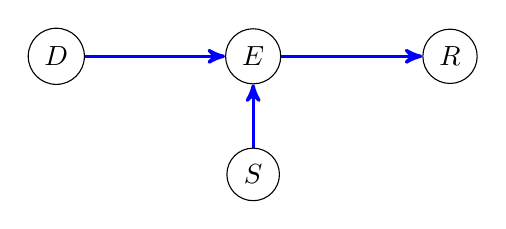
\begin{tikzpicture}[->,>=stealth']
    \tikzstyle{every state}=[draw=none]
    \node[shape=circle, draw] (D) at (0,0) {$D$};
    \node[shape=circle, draw] (E) at (2.5,0) {$E$};
    \node[shape=circle, draw] (R) at (5,0) {$R$};
    \node[shape=circle, draw] (S) at (2.5,-1.5) {$S$};
    
      \path 
    	(D)  edge  [very thick, color=blue]    (E)  
  %  	(A)  edge  [bend left,very thick, color=blue]  (Y)
    	(E)  edge  [very thick, color=blue]  (R)		
    	(S) edge  [very thick, color=blue]  (E)
    	;
    \end{tikzpicture}
    \end{center}
    
        \caption{Dose response relationship that is completely mediated by exposure, with PK difference between adult and pediatric}
\end{figure}



\begin{figure}[H]
    \begin{center}
    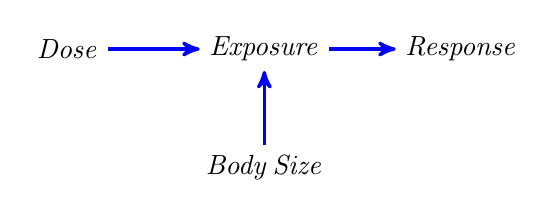
\begin{tikzpicture}[->,>=stealth']
    \tikzstyle{every state}=[draw=none]
    \node[] (D) at (0,0) {$\mathit{Dose}$};
    \node[] (E) at (2.5,0) {$\mathit{Exposure}$};
    \node[] (R) at (5,0) {$\mathit{Response}$};
    \node[] (W) at (2.5,-1.5) {$\mathit{Body \, Size}$};
    
      \path 
    	(D)  edge  [very thick, color=blue]    (E)  
  %  	(A)  edge  [bend left,very thick, color=blue]  (Y)
    	(E)  edge  [very thick, color=blue]  (R)		
    	(W) edge  [very thick, color=blue]  (E)
    	;
    \end{tikzpicture}
    \end{center}
    
        \caption{Full extrapolation with allometrically scaled PK}
\end{figure}

\begin{figure}[H]
    \begin{center}
    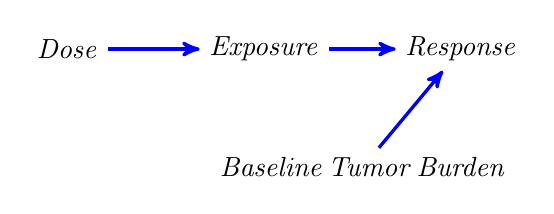
\begin{tikzpicture}[->,>=stealth']
    \tikzstyle{every state}=[draw=none]
    \node[] (D) at (0,0) {$\mathit{Dose}$};
    \node[] (E) at (2.5,0) {$\mathit{Exposure}$};
    \node[] (R) at (5,0) {$\mathit{Response}$};
    \node[] (W) at (3.75,-1.5) {$\mathit{Baseline \, Tumor \, Burden}$};
    
      \path 
    	(D)  edge  [very thick, color=blue]    (E)  
  %  	(A)  edge  [bend left,very thick, color=blue]  (Y)
    	(E)  edge  [very thick, color=blue]  (R)	
    	(W) edge  [very thick, color=blue]  (R)
    %	(W) edge  [very thick, color=blue]  (E)
    	;
    \end{tikzpicture}
    \end{center}
    
        \caption{Trastuzumab Naive}
\end{figure}


\begin{figure}[H]
    \begin{center}
    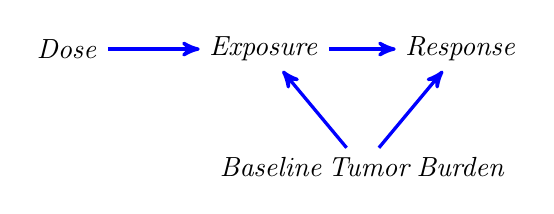
\begin{tikzpicture}[->,>=stealth']
    \tikzstyle{every state}=[draw=none]
    \node[] (D) at (0,0) {$\mathit{Dose}$};
    \node[] (E) at (2.5,0) {$\mathit{Exposure}$};
    \node[] (R) at (5,0) {$\mathit{Response}$};
    \node[] (W) at (3.75,-1.5) {$\mathit{Baseline \, Tumor \, Burden}$};
    
      \path 
    	(D)  edge  [very thick, color=blue]    (E)  
  %  	(A)  edge  [bend left,very thick, color=blue]  (Y)
    	(E)  edge  [very thick, color=blue]  (R)	
    	(W) edge  [very thick, color=blue]  (R)
    	(W) edge  [very thick, color=blue]  (E)
    	;
    \end{tikzpicture}
    \end{center}
    
        \caption{Trastuzumab}
\end{figure}

\begin{figure}[H]
    \begin{center}
    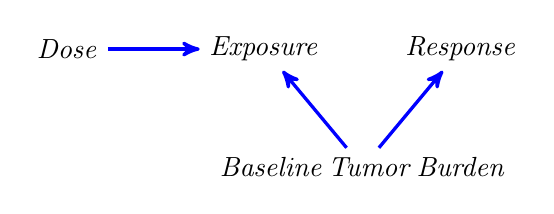
\begin{tikzpicture}[->,>=stealth']
    \tikzstyle{every state}=[draw=none]
    \node[] (D) at (0,0) {$\mathit{Dose}$};
    \node[] (E) at (2.5,0) {$\mathit{Exposure}$};
    \node[] (R) at (5,0) {$\mathit{Response}$};
    \node[] (W) at (3.75,-1.5) {$\mathit{Baseline \, Tumor \, Burden}$};
    
      \path 
    	(D)  edge  [very thick, color=blue]    (E)  
  %  	(A)  edge  [bend left,very thick, color=blue]  (Y)
    	% (E)  edge  [very thick, color=blue]  (R)	
    	(W) edge  [very thick, color=blue]  (R)
    	(W) edge  [very thick, color=blue]  (E)
    	;
    \end{tikzpicture}
    \end{center}
    
        \caption{Trastuzumab post hoc}
\end{figure}


\begin{figure}[H]
    \begin{center}
    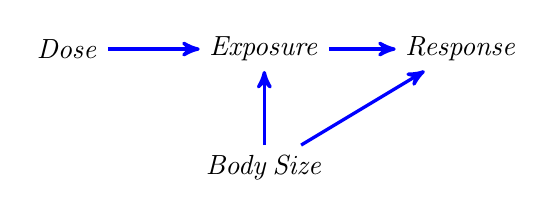
\begin{tikzpicture}[->,>=stealth']
    \tikzstyle{every state}=[draw=none]
    \node[] (D) at (0,0) {$\mathit{Dose}$};
    \node[] (E) at (2.5,0) {$\mathit{Exposure}$};
    \node[] (R) at (5,0) {$\mathit{Response}$};
    \node[] (W) at (2.5,-1.5) {$\mathit{Body \, Size}$};
    
      \path 
    	(D)  edge  [very thick, color=blue]    (E)  
  %  	(A)  edge  [bend left,very thick, color=blue]  (Y)
    	(E)  edge  [very thick, color=blue]  (R)	
    	(W) edge  [very thick, color=blue]  (R)
    	(W) edge  [very thick, color=blue]  (E)
    	;
    \end{tikzpicture}
    \end{center}
    
        \caption{SGLT-2}
\end{figure}



\begin{figure}[H]
    \begin{center}
    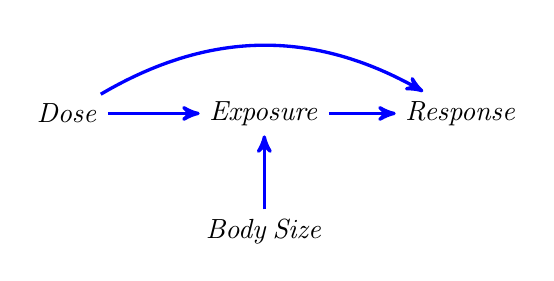
\begin{tikzpicture}[->,>=stealth']
    \tikzstyle{every state}=[draw=none]
    \node[] (D) at (0,0) {$\mathit{Dose}$};
    \node[] (E) at (2.5,0) {$\mathit{Exposure}$};
    \node[] (R) at (5,0) {$\mathit{Response}$};
    \node[] (W) at (2.5,-1.5) {$\mathit{Body \, Size}$};
    %\node[] (U1) at (0,-1.5) {$\mathit{U_1}$};
    %\node[] (U2) at (5,-1.5) {$\mathit{Confounder}$};
    
      \path 
    	(D)  edge  [very thick, color=blue]    (E)  
    	(D)  edge  [bend left,very thick, color=blue]  (R)
    	(E)  edge  [very thick, color=blue]  (R)		
    	(W) edge  [very thick, color=blue]  (E)
    	%(U1) edge  [very thick, color=grapefruit, dashed]  (E)
    	%(U2) edge  [very thick, color=pine, dashed]  (E)
    	%(U2) edge  [very thick, color=pine, dashed]  (R)
    	;
    \end{tikzpicture}
    \end{center}
    
        \caption{Questions before full extrapolation with allometric scaling}
\end{figure}


\begin{figure}[H]
    \begin{center}
    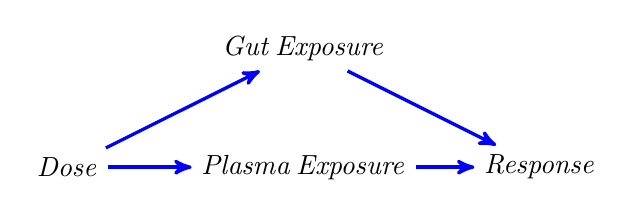
\begin{tikzpicture}[->,>=stealth']
    \tikzstyle{every state}=[draw=none]
    \node[] (D) at (0,0) {$\mathit{Dose}$};
    \node[] (E) at (3,0) {$\mathit{Plasma \, Exposure}$};
    \node[] (E2) at (3,1.5) {$\mathit{Gut \, Exposure}$};
    \node[] (R) at (6,0) {$\mathit{Response}$};
    %\node[] (W) at (3,-1.5) {$\mathit{Body \, Size}$};
    %\node[] (U1) at (0,-1.5) {$\mathit{U_1}$};
    %\node[] (U2) at (5,-1.5) {$\mathit{Confounder}$};
    
      \path 
    	(D)  edge  [very thick, color=blue]    (E)  
    	(D)  edge  [very thick, color=blue]  (E2)
    	(E2)  edge  [very thick, color=blue]  (R)
    	(E)  edge  [very thick, color=blue]  (R)		
    	%(W) edge  [very thick, color=blue]  (E)
    	%(U1) edge  [very thick, color=grapefruit, dashed]  (E)
    	%(U2) edge  [very thick, color=pine, dashed]  (E)
    	%(U2) edge  [very thick, color=pine, dashed]  (R)
    	;
    \end{tikzpicture}
    \end{center}
    
        \caption{Show mediator?}
\end{figure}


\begin{figure}[H]
    \begin{center}
    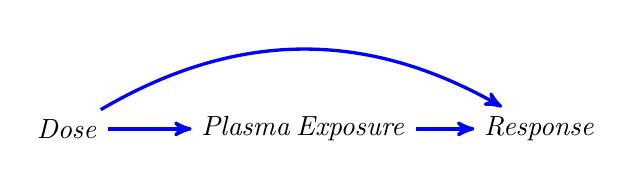
\begin{tikzpicture}[->,>=stealth']
    \tikzstyle{every state}=[draw=none]
    \node[] (D) at (0,0) {$\mathit{Dose}$};
    \node[] (E) at (3,0) {$\mathit{Plasma \, Exposure}$};
    \node[] (R) at (6,0) {$\mathit{Response}$};
    % \node[] (W) at (3,-1.5) {$\mathit{Body \, Size}$};
    %\node[] (U1) at (0,-1.5) {$\mathit{U_1}$};
    %\node[] (U2) at (5,-1.5) {$\mathit{Confounder}$};
    
      \path 
    	(D)  edge  [very thick, color=blue]    (E)  
    	(D)  edge  [bend left,very thick, color=blue]  (R)
    	(E)  edge  [very thick, color=blue]  (R)		
    	% (W) edge  [very thick, color=blue]  (E)
    	%(U1) edge  [very thick, color=grapefruit, dashed]  (E)
    	%(U2) edge  [very thick, color=pine, dashed]  (E)
    	%(U2) edge  [very thick, color=pine, dashed]  (R)
    	;
    \end{tikzpicture}
    \end{center}
    
        \caption{Or not?}
\end{figure}


\begin{figure}[H]
    \begin{center}
    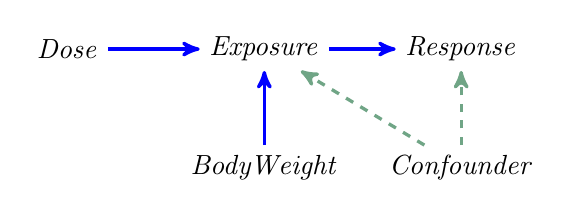
\begin{tikzpicture}[->,>=stealth']
    \tikzstyle{every state}=[draw=none]
    \node[] (D) at (0,0) {$\mathit{Dose}$};
    \node[] (E) at (2.5,0) {$\mathit{Exposure}$};
    \node[] (R) at (5,0) {$\mathit{Response}$};
    \node[] (W) at (2.5,-1.5) {$\mathit{Body Weight}$};
    %\node[] (U1) at (0,-1.5) {$\mathit{U_1}$};
    \node[] (U2) at (5,-1.5) {$\mathit{Confounder}$};
    
      \path 
    	(D)  edge  [very thick, color=blue]    (E)  
    	% (D)  edge  [bend left,very thick, color=bark, dashed]  (R)
    	(E)  edge  [very thick, color=blue]  (R)		
    	(W) edge  [very thick, color=blue]  (E)
    	%(U1) edge  [very thick, color=grapefruit, dashed]  (E)
    	(U2) edge  [very thick, color=pine, dashed]  (E)
    	(U2) edge  [very thick, color=pine, dashed]  (R)
    	;
    \end{tikzpicture}
    \end{center}
    
        \caption{More questions before full extrapolation with allometric scaling}
\end{figure}


$D \independent R^{(d)} \,\,\, | \,\,\, E$

$D \not\!\perp\!\!\!\perp R^{(d)} \,\,\, | \,\,\, E$

\begin{figure}[H]
    \begin{center}
    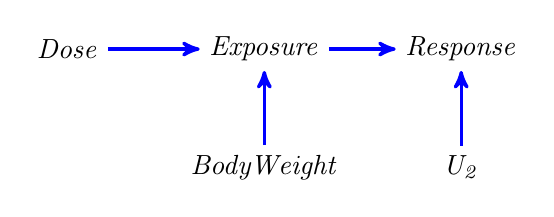
\begin{tikzpicture}[->,>=stealth']
    \tikzstyle{every state}=[draw=none]
    \node[] (D) at (0,0) {$\mathit{Dose}$};
    \node[] (E) at (2.5,0) {$\mathit{Exposure}$};
    \node[] (R) at (5,0) {$\mathit{Response}$};
    \node[] (W) at (2.5,-1.5) {$\mathit{Body Weight}$};
    % \node[] (U1) at (0,-1.5) {$\mathit{U_1}$};
    \node[] (U2) at (5,-1.5) {$\mathit{U_2}$};
    
      \path 
    	(D)  edge  [very thick, color=blue]    (E)  
    	% (D)  edge  [bend left,very thick, color=bark, dashed]  (R)
    	(E)  edge  [very thick, color=blue]  (R)		
    	(W) edge  [very thick, color=blue]  (E)
    	% (U1) edge  [very thick, color=blue]  (E)
    	% (U2) edge  [very thick, color=pine, dashed]  (E)
    	(U2) edge  [very thick, color=blue]  (R)
    	;
    \end{tikzpicture}
    \end{center}
    
        \caption{Working DAG within adults and within peds}
\end{figure}


\begin{figure}[H]
    \begin{center}
    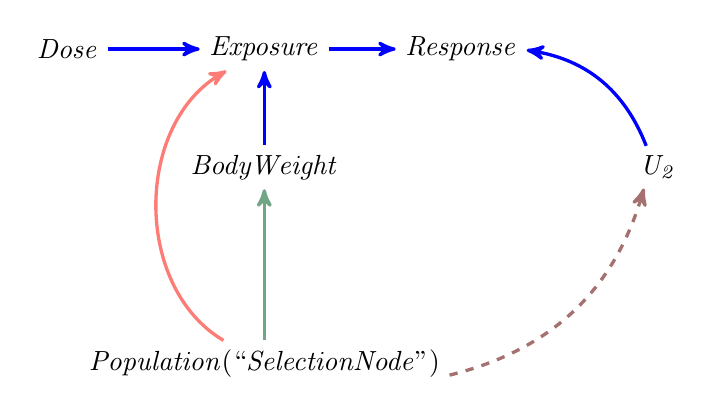
\begin{tikzpicture}[->,>=stealth']
    \tikzstyle{every state}=[draw=none]
    \node[] (D) at (0,0) {$\mathit{Dose}$};
    \node[] (E) at (2.5,0) {$\mathit{Exposure}$};
    \node[] (R) at (5,0) {$\mathit{Response}$};
    \node[] (W) at (2.5,-1.5) {$\mathit{Body Weight}$};
    %\node[] (U1) at (0,-1.5) {$\mathit{U_1}$};
    \node[] (U2) at (7.5,-1.5) {$\mathit{U_2}$};
    \node[] (S) at (2.5,-4) {$\mathit{Population (``Selection Node")}$};
    
      \path 
    	(D)  edge  [very thick, color=blue]    (E)  
    	% (D)  edge  [bend left,very thick, color=bark, dashed]  (R)
    	(E)  edge  [very thick, color=blue]  (R)		
    	(W) edge  [very thick, color=blue]  (E)
    	% (U1) edge  [very thick, color=blue]  (E)
    	% (U2) edge  [very thick, color=pine, dashed]  (E)
    	(U2) edge  [very thick, color=blue, bend right]  (R)
    	(S) edge  [bend left=60, very thick, color=grapefruit]  (E)
    	(S) edge  [very thick, color=pine]  (W)
    	(S) edge  [very thick, color=blue, bend right, color=bark, dashed]  (U2)
    	;
    \end{tikzpicture}
    \end{center}
    
        \caption{Selection graph for full extrapolation: justification}
\end{figure}



\begin{figure}[H]
    \begin{center}
    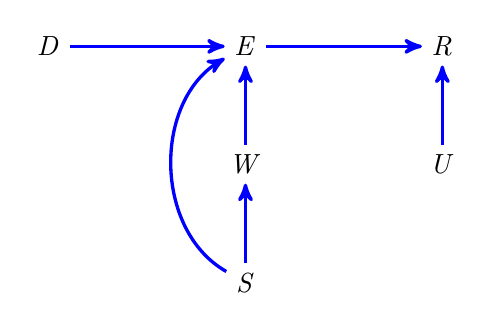
\begin{tikzpicture}[->,>=stealth']
    \tikzstyle{every state}=[draw=none]
    \node[] (D) at (0,0) {$\mathit{D}$};
    \node[] (E) at (2.5,0) {$\mathit{E}$};
    \node[] (R) at (5,0) {$\mathit{R}$};
    \node[] (W) at (2.5,-1.5) {$\mathit{W}$};
    %\node[] (U1) at (0,-1.5) {$\mathit{U_1}$};
    \node[] (U2) at (5,-1.5) {$\mathit{U}$};
    \node[] (S) at (2.5,-3) {$\mathit{S}$};
    
      \path 
    	(D)  edge  [very thick, color=blue]    (E)  
    	% (D)  edge  [bend left,very thick, color=bark, dashed]  (R)
    	(E)  edge  [very thick, color=blue]  (R)		
    	(W) edge  [very thick, color=blue]  (E)
    	% (U1) edge  [very thick, color=blue]  (E)
    	% (U2) edge  [very thick, color=pine, dashed]  (E)
    	(U2) edge  [very thick, color=blue]  (R)
    	(S) edge  [bend left=60, very thick, color=blue]  (E)
    	(S) edge  [very thick, color=blue]  (W)
    	;
    \end{tikzpicture}
    \end{center}
    
        \caption{Working selection diagram for full extrapolation.}
\end{figure}


\begin{displaymath}
\begin{array}{rl}
D &= \mbox{dose or treatment status}  \\
E &= \mbox{exposure (summary metric)}  \\
R &= \mbox{Response} \\
W &= \mbox{Body weight} \\
U &= \mbox{Unmeasured effect modifier} \\
S &= \mbox{Selection node (pediatric status)}
\end{array}
\end{displaymath}
 


\begin{displaymath}
\begin{array}{|l|c|c|}
\hline
& \mbox{Adult} & \mbox{Pediatric} \\ \hline
\mbox{Observational} & P(\bm{v} | D=d)     & P^*(\bm{v} | D=d) \\ \hline
\mbox{Interventional} & P(\bm{v} | \mathrm{do}(D = d))     & P^*(\bm{v}| \mathrm{do}(D = d)) \\ \hline
\end{array}
\end{displaymath}


$$ P^*(r| \mathrm{do}(D = d)) $$ 

\begin{align} 
P(r \, | \, \mathrm{do}(D=d)) &= \int_e P^*(r \,|\, e, \mathrm{do}(D=d)) P^*(e \,|\, \mathrm{do}(D=d)) \\
&= \int_e P^*(r \,|\, e) P^*(e \,|\, \mathrm{do}(D=d))
\end{align}


\begin{displaymath}
\begin{array}{rlr}
P^*(r \, | \, \mathrm{do}(D=d)) &= \int_e P^*(r \,|\, e, \mathrm{do}(D=d)) P^*(e \,|\, \mathrm{do}(D=d))\mathrm{d}e & \mbox{(Law of total prb.)} \\
&= \int_e P^*(r \,|\, e) P^*(e \,|\, \mathrm{do}(D=d))\mathrm{d}e & (D \perp R \,|\, E)  \\
&= \int_e P(r \,|\, e) P^*(e \,|\, \mathrm{do}(D=d))\mathrm{d}e & (S \perp R \,|\, E) \\
\end{array}
\end{displaymath}




\begin{figure}[H]
    \begin{center}
    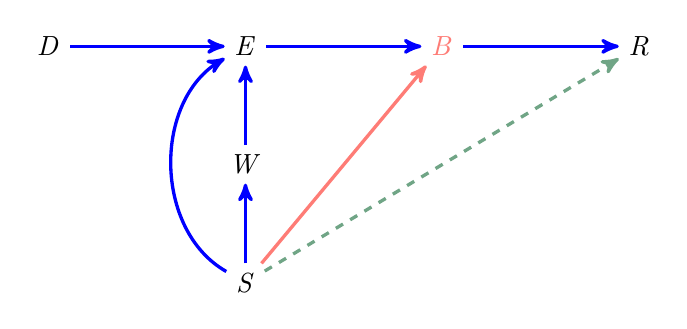
\begin{tikzpicture}[->,>=stealth']
    \tikzstyle{every state}=[draw=none]
    \node[] (D) at (0,0) {$\mathit{D}$};
    \node[] (E) at (2.5,0) {$\mathit{E}$};
    \node[] (B) at (5,0) {$\color{grapefruit} \mathit{B}$};
    \node[] (R) at (7.5,0) {$\mathit{R}$};
    \node[] (W) at (2.5,-1.5) {$\mathit{W}$};
    %\node[] (U1) at (0,-1.5) {$\mathit{U_1}$};
    %\node[] (U2) at (7.5,-1.5) {$\mathit{U}$};
    \node[] (S) at (2.5,-3) {$\mathit{S}$};
    
      \path 
    	(D)  edge  [very thick, color=blue]    (E)  
    	% (D)  edge  [bend left,very thick, color=bark, dashed]  (R)
    	(E)  edge  [very thick, color=blue]  (B)		
    	(B)  edge  [very thick, color=blue]  (R)		
    	(W) edge  [very thick, color=blue]  (E)
    	% (U1) edge  [very thick, color=blue]  (E)
    	% (U2) edge  [very thick, color=pine, dashed]  (E)
    	% (U2) edge  [very thick, color=blue]  (R)
    	(S) edge  [bend left=60, very thick, color=blue]  (E)
    	(S) edge  [very thick, color=blue]  (W)
    	(S) edge  [very thick, color=grapefruit]  (B)
    	(S) edge  [very thick, color=pine, dashed]  (R)
    	;
    \end{tikzpicture}
    \end{center}
    
        \caption{Working selection diagram for full bridging biomarker.}
\end{figure}


\begin{figure}[H]
    \begin{center}
    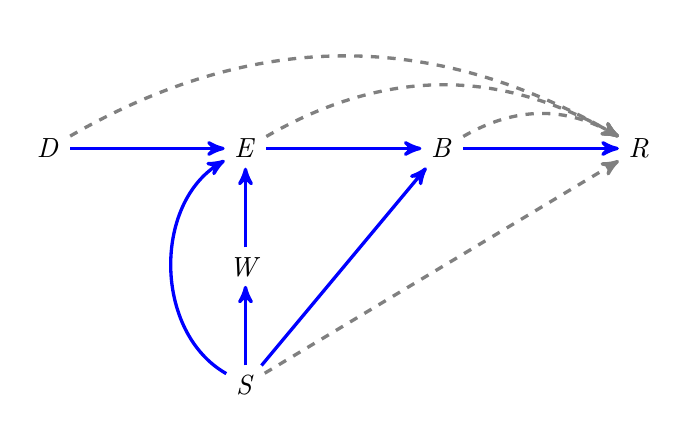
\begin{tikzpicture}[->,>=stealth']
    \tikzstyle{every state}=[draw=none]
    \node[] (D) at (0,0) {$\mathit{D}$};
    \node[] (E) at (2.5,0) {$\mathit{E}$};
    \node[] (B) at (5,0) {$\mathit{B}$};
    \node[] (R) at (7.5,0) {$\mathit{R}$};
    \node[] (W) at (2.5,-1.5) {$\mathit{W}$};
    %\node[] (U1) at (0,-1.5) {$\mathit{U_1}$};
    %\node[] (U2) at (7.5,-1.5) {$\mathit{U}$};
    \node[] (S) at (2.5,-3) {$\mathit{S}$};
    
      \path 
    	(D)  edge  [very thick, color=blue]    (E)  
    	% (D)  edge  [bend left,very thick, color=bark, dashed]  (R)
    	(E)  edge  [very thick, color=blue]  (B)		
    	(B)  edge  [very thick, color=blue]  (R)		
    	(W) edge  [very thick, color=blue]  (E)
    	% (U1) edge  [very thick, color=blue]  (E)
    	% (U2) edge  [very thick, color=pine, dashed]  (E)
    	% (U2) edge  [very thick, color=blue]  (R)
    	(S) edge  [bend left=60, very thick, color=blue]  (E)
    	(S) edge  [very thick, color=blue]  (W)
    	(S) edge  [very thick, color=blue]  (B)
    	(S) edge  [very thick, color=gray, dashed]  (R)
    	(B) edge  [very thick, color=gray, bend left, dashed]  (R)
    	(E) edge  [very thick, color=gray, bend left, dashed]  (R)
    	(D) edge  [very thick, color=gray, bend left, dashed]  (R)
    	;
    \end{tikzpicture}
    \end{center}
    
        \caption{Bridging biomarker selection diagram that could be wrong}
\end{figure}



\begin{displaymath}
\begin{array}{rlr}
P^*(r \, | \, \mathrm{do}(D=d)) &= \int_b P^*(r \,|\, b, \mathrm{do}(D=d)) P^*(b \,|\, \mathrm{do}(D=d))\mathrm{d}b & \mbox{(Law of total prb.)} \\
&= \int_b P^*(r \,|\, b) P^*(b \,|\, do(D=d))\mathrm{d}b & (D \perp R \,|\, B)  \\
&= \int_b P(r \,|\, b) P^*(b \,|\, do(D=d))\mathrm{d}b & (S \perp R \,|\, B) \\
\end{array}
\end{displaymath}

%%%%%%%%%%%%%%%%%%%%%%%%%%%%%%%



\begin{figure}[H]
    \begin{center}
    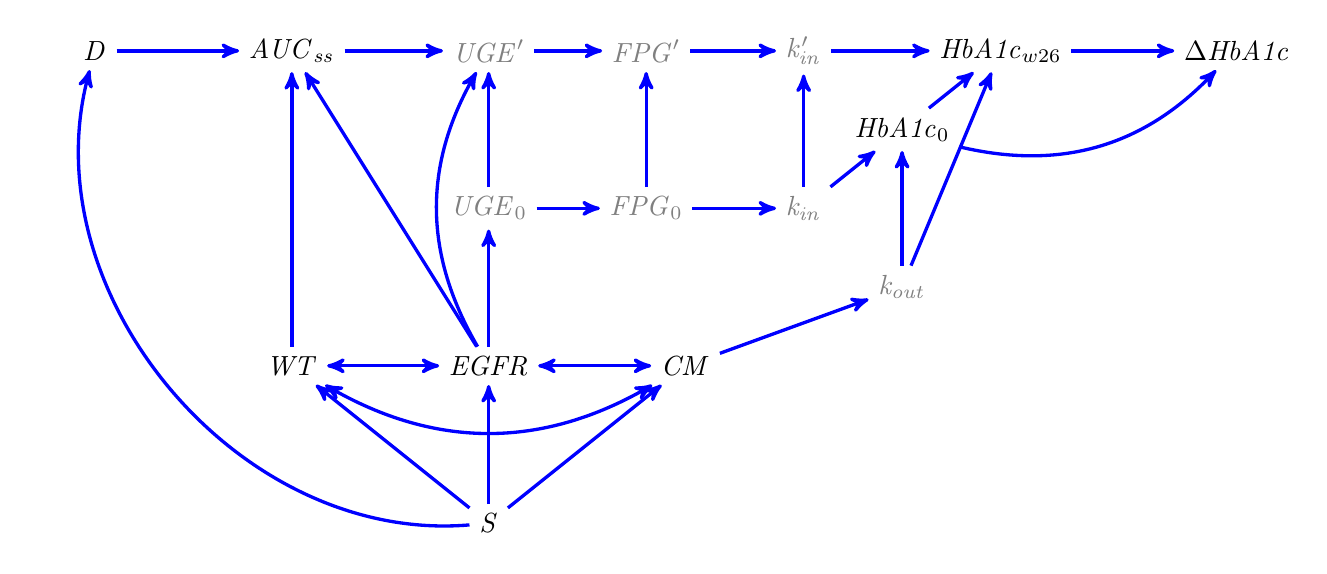
\begin{tikzpicture}[->,>=stealth']
    \tikzstyle{every state}=[draw=none]
    \node[] (D) at (0,0) {$\mathit{D}$};
    \node[] (AUC) at (2.5,0) {$\mathit{AUC}_\mathit{ss}$};
    \node[] (UGE) at (5,0) {$\color{gray} \mathit{UGE}'$};
    \node[] (UGE0) at (5,-2) {$\color{gray} \mathit{UGE}_0$};
    \node[] (FPG) at (7,0) {$\color{gray} \mathit{FPG}'$};
    \node[] (FPG0) at (7,-2) {$\color{gray} \mathit{FPG}_0$};
    \node[] (kinprime) at (9,0) {$\color{gray} \mathit{k'_{\mathit{in}}}$};
    \node[] (kin) at (9,-2) {$\color{gray} \mathit{k_{\mathit{in}}}$};
    \node[] (kout) at (10.25,-3) {$\color{gray} \mathit{k_{\mathit{out}}}$};
    \node[] (R) at (11.5,0) {$\mathit{HbA1c}_{w26}$};
    \node[] (R0) at (10.25,-1) {$\mathit{HbA1c}_0$};
    \node[] (WT) at (2.5,-4) {$\mathit{WT}$};
    \node[] (EGFR) at (5,-4) {$\mathit{EGFR}$};
    \node[] (CM) at (7.5,-4) {$\mathit{CM}$};
    \node[] (S) at (5,-6) {$\mathit{S}$};
    \node[] (delta) at (14.5,0) {$\Delta\mathit{HbA1c}$};
    
      \path 
    	(D)  edge  [very thick, color=blue]    (AUC)  
    	(AUC)  edge  [very thick, color=blue]  (UGE)		
    	(FPG)  edge  [very thick, color=blue]  (kinprime)		
    	(kinprime)  edge  [very thick, color=blue]  (R)		
    	
    	(WT) edge  [very thick, color=blue]  (AUC)
    	(EGFR) edge  [very thick, color=blue]  (AUC)
    	(EGFR) edge  [very thick, color=blue]  (UGE0)
    	(EGFR) edge  [very thick, color=blue, bend left]  (UGE)
    	(UGE0) edge  [very thick, color=blue]  (UGE)
    	(UGE0) edge  [very thick, color=blue]  (FPG0)
    	(UGE) edge  [very thick, color=blue]  (FPG)
    	(FPG0) edge  [very thick, color=blue]  (FPG)
    	(FPG0) edge  [very thick, color=blue]  (kin)
    	(kin) edge  [very thick, color=blue]  (kinprime)
    	(kin) edge  [very thick, color=blue]  (R0)
    	(kout) edge  [very thick, color=blue]  (R0)
    	(kout) edge  [very thick, color=blue]  (R)
    	(CM) edge  [very thick, color=blue]  (kout)
      (R0) edge  [very thick, color=blue]  (R)
      (R0) edge  [very thick, color=blue, bend right]  (delta)
      (R) edge  [very thick, color=blue]  (delta)
      
          	(WT) edge[<->, very thick, color=blue] (EGFR)
    	(CM) edge[<->, very thick, color=blue] (EGFR)
    	(WT) edge[<->, very thick, color=blue, bend right] (CM)

    	% (S) edge  [bend left=60, very thick, color=blue]  (E)
    	(S) edge  [very thick, color=blue]  (WT)
    	(S) edge  [very thick, color=blue]  (EGFR)
    	(S) edge  [very thick, color=blue]  (CM)
    	(S) edge  [very thick, color=blue, bend left=55]  (D)
    	;
    \end{tikzpicture}
    \end{center}
    
        \caption{DINAMO Selection Diagram}
\end{figure}


\begin{displaymath}
\begin{array}{rl}
D &= \mbox{dose or treatment status}  \\
AUC_\mathit{ss} &= \mbox{exposure at PK steady-state}  \\
UGE_0, UGE' &= \mbox{urinary glucose excretion, pre- and post-treatment}  \\
FPG_0, FPG' &= \mbox{fasting plasma glucose, pre- and post-treatment}  \\
k_\mathit{in}, k'_\mathit{in} &= \mbox{rate constant for HbA1c synthesis, pre- and post-treatment}  \\
k_\mathit{out} &= \mbox{rate constant for HbA1c degradation / elimination}  
\end{array}
\end{displaymath}


\begin{displaymath}
\begin{array}{rl}
\mathit{HbA1c}_0, \mathit{HbA1c}_{w26} &= \mbox{hemoglobin A1c at baseline and week 26} \\
\mathit{\Delta HbA1c} &= \mbox{Change from baseline in hemoglobin A1c} \\
WT &= \mbox{Body weight} \\
EGFR &= \mbox{estimated glomerular filtration rate} \\
CM &= \mbox{Concomitant medication usage} \\
S &= \mbox{Selection node (pediatric status)}
\end{array}
\end{displaymath}




\begin{figure}[H]
    \begin{center}
    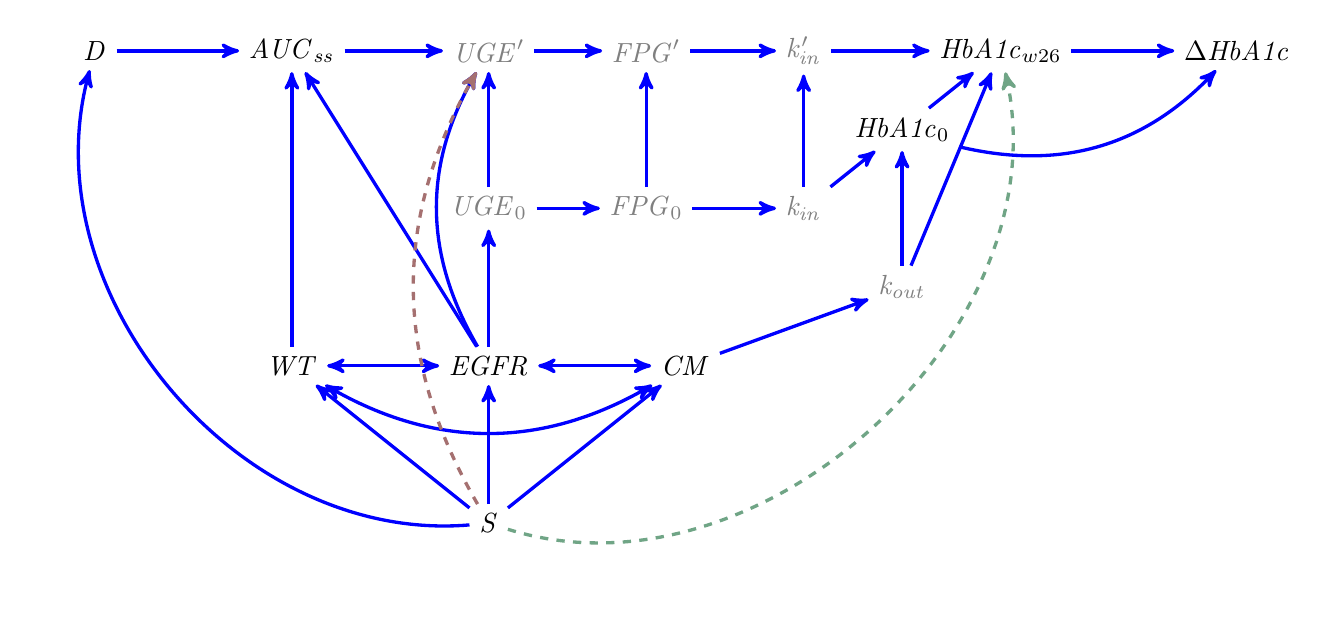
\begin{tikzpicture}[->,>=stealth']
    \tikzstyle{every state}=[draw=none]
    \node[] (D) at (0,0) {$\mathit{D}$};
    \node[] (AUC) at (2.5,0) {$\mathit{AUC}_\mathit{ss}$};
    \node[] (UGE) at (5,0) {$\color{gray} \mathit{UGE}'$};
    \node[] (UGE0) at (5,-2) {$\color{gray} \mathit{UGE}_0$};
    \node[] (FPG) at (7,0) {$\color{gray} \mathit{FPG}'$};
    \node[] (FPG0) at (7,-2) {$\color{gray} \mathit{FPG}_0$};
    \node[] (kinprime) at (9,0) {$\color{gray} \mathit{k'_{\mathit{in}}}$};
    \node[] (kin) at (9,-2) {$\color{gray} \mathit{k_{\mathit{in}}}$};
    \node[] (kout) at (10.25,-3) {$\color{gray} \mathit{k_{\mathit{out}}}$};
    \node[] (R) at (11.5,0) {$\mathit{HbA1c}_{w26}$};
    \node[] (R0) at (10.25,-1) {$\mathit{HbA1c}_0$};
    \node[] (WT) at (2.5,-4) {$\mathit{WT}$};
    \node[] (EGFR) at (5,-4) {$\mathit{EGFR}$};
    \node[] (CM) at (7.5,-4) {$\mathit{CM}$};
    \node[] (S) at (5,-6) {$\mathit{S}$};
    \node[] (delta) at (14.5,0) {$\Delta\mathit{HbA1c}$};
    
      \path 
    	(D)  edge  [very thick, color=blue]    (AUC)  
    	(AUC)  edge  [very thick, color=blue]  (UGE)		
    	(FPG)  edge  [very thick, color=blue]  (kinprime)		
    	(kinprime)  edge  [very thick, color=blue]  (R)		
    	
    	(WT) edge  [very thick, color=blue]  (AUC)
    	(EGFR) edge  [very thick, color=blue]  (AUC)
    	(EGFR) edge  [very thick, color=blue]  (UGE0)
    	(EGFR) edge  [very thick, color=blue, bend left]  (UGE)
    	(UGE0) edge  [very thick, color=blue]  (UGE)
    	(UGE0) edge  [very thick, color=blue]  (FPG0)
    	(UGE) edge  [very thick, color=blue]  (FPG)
    	(FPG0) edge  [very thick, color=blue]  (FPG)
    	(FPG0) edge  [very thick, color=blue]  (kin)
    	(kin) edge  [very thick, color=blue]  (kinprime)
    	(kin) edge  [very thick, color=blue]  (R0)
    	(kout) edge  [very thick, color=blue]  (R0)
    	(kout) edge  [very thick, color=blue]  (R)
    	(CM) edge  [very thick, color=blue]  (kout)
      (R0) edge  [very thick, color=blue]  (R)
      (R0) edge  [very thick, color=blue, bend right]  (delta)
      (R) edge  [very thick, color=blue]  (delta)
      
                	(WT) edge[<->, very thick, color=blue] (EGFR)
    	(CM) edge[<->, very thick, color=blue] (EGFR)
    	(WT) edge[<->, very thick, color=blue, bend right] (CM)

    	% (S) edge  [bend left=60, very thick, color=blue]  (E)
    	(S) edge  [very thick, color=blue]  (WT)
    	(S) edge  [very thick, color=blue]  (EGFR)
    	(S) edge  [very thick, color=blue]  (CM)
    	(S) edge  [very thick, color=blue, bend left=55]  (D)
    	
    	(S) edge  [very thick, color=bark, dashed, bend left]  (UGE)
    	(S) edge  [very thick, color=pine, dashed, bend right=60]  (R)
    	;
    \end{tikzpicture}
    \end{center}
    
        \caption{DINAMO Selection Diagram}
\end{figure}




\begin{figure}[H]
    \begin{center}
    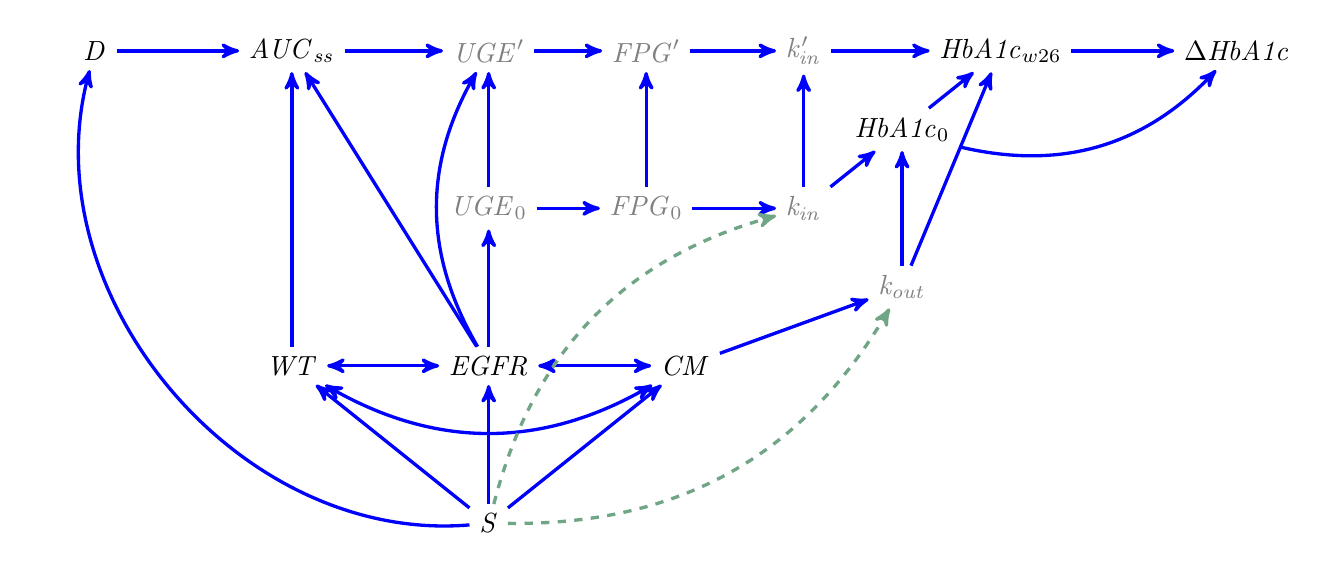
\begin{tikzpicture}[->,>=stealth']
    \tikzstyle{every state}=[draw=none]
    \node[] (D) at (0,0) {$\mathit{D}$};
    \node[] (AUC) at (2.5,0) {$\mathit{AUC}_\mathit{ss}$};
    \node[] (UGE) at (5,0) {$\color{gray} \mathit{UGE}'$};
    \node[] (UGE0) at (5,-2) {$\color{gray} \mathit{UGE}_0$};
    \node[] (FPG) at (7,0) {$\color{gray} \mathit{FPG}'$};
    \node[] (FPG0) at (7,-2) {$\color{gray} \mathit{FPG}_0$};
    \node[] (kinprime) at (9,0) {$\color{gray} \mathit{k'_{\mathit{in}}}$};
    \node[] (kin) at (9,-2) {$\color{gray} \mathit{k_{\mathit{in}}}$};
    \node[] (kout) at (10.25,-3) {$\color{gray} \mathit{k_{\mathit{out}}}$};
    \node[] (R) at (11.5,0) {$\mathit{HbA1c}_{w26}$};
    \node[] (R0) at (10.25,-1) {$\mathit{HbA1c}_0$};
    \node[] (WT) at (2.5,-4) {$\mathit{WT}$};
    \node[] (EGFR) at (5,-4) {$\mathit{EGFR}$};
    \node[] (CM) at (7.5,-4) {$\mathit{CM}$};
    \node[] (S) at (5,-6) {$\mathit{S}$};
    \node[] (delta) at (14.5,0) {$\Delta\mathit{HbA1c}$};
    
      \path 
    	(D)  edge  [very thick, color=blue]    (AUC)  
    	(AUC)  edge  [very thick, color=blue]  (UGE)		
    	(FPG)  edge  [very thick, color=blue]  (kinprime)		
    	(kinprime)  edge  [very thick, color=blue]  (R)		
    	
    	(WT) edge  [very thick, color=blue]  (AUC)
    	(EGFR) edge  [very thick, color=blue]  (AUC)
    	(EGFR) edge  [very thick, color=blue]  (UGE0)
    	(EGFR) edge  [very thick, color=blue, bend left]  (UGE)
    	(UGE0) edge  [very thick, color=blue]  (UGE)
    	(UGE0) edge  [very thick, color=blue]  (FPG0)
    	(UGE) edge  [very thick, color=blue]  (FPG)
    	(FPG0) edge  [very thick, color=blue]  (FPG)
    	(FPG0) edge  [very thick, color=blue]  (kin)
    	(kin) edge  [very thick, color=blue]  (kinprime)
    	(kin) edge  [very thick, color=blue]  (R0)
    	(kout) edge  [very thick, color=blue]  (R0)
    	(kout) edge  [very thick, color=blue]  (R)
    	(CM) edge  [very thick, color=blue]  (kout)
      (R0) edge  [very thick, color=blue]  (R)
      (R0) edge  [very thick, color=blue, bend right]  (delta)
      (R) edge  [very thick, color=blue]  (delta)
      
      (WT) edge[<->, very thick, color=blue] (EGFR)
    	(CM) edge[<->, very thick, color=blue] (EGFR)
    	(WT) edge[<->, very thick, color=blue, bend right] (CM)

    	% (S) edge  [bend left=60, very thick, color=blue]  (E)
    	(S) edge  [very thick, color=blue]  (WT)
    	(S) edge  [very thick, color=blue]  (EGFR)
    	(S) edge  [very thick, color=blue]  (CM)
    	(S) edge  [very thick, color=blue, bend left=55]  (D)
    	
    	(S) edge  [very thick, color=pine, dashed, bend left=30]  (kin)
    	(S) edge  [very thick, color=pine, dashed, bend right]  (kout)
    	
    	;
    \end{tikzpicture}
    \end{center}
    
        \caption{DINAMO Selection Diagram}
\end{figure}

\begin{figure}[H]
    \begin{center}
    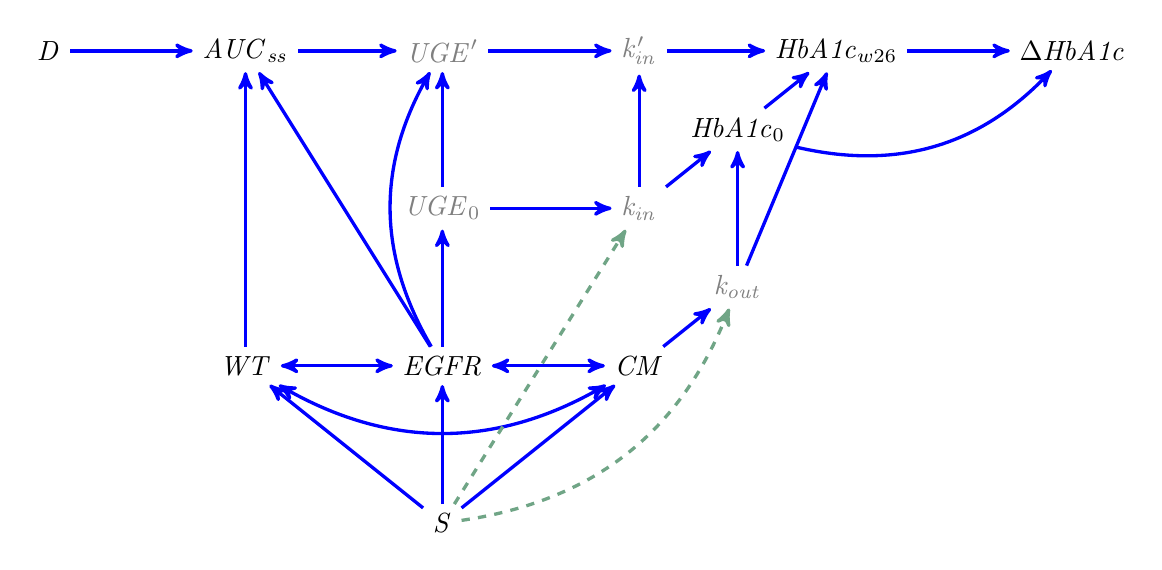
\begin{tikzpicture}[->,>=stealth']
    \tikzstyle{every state}=[draw=none]
    \node[] (D) at (0,0) {$\mathit{D}$};
    \node[] (AUC) at (2.5,0) {$\mathit{AUC}_\mathit{ss}$};
    \node[] (UGE) at (5,0) {$\color{gray} \mathit{UGE}'$};
    \node[] (UGE0) at (5,-2) {$\color{gray} \mathit{UGE}_0$};
    \node[] (kinprime) at (7.5,0) {$\color{gray} \mathit{k'_{\mathit{in}}}$};
    \node[] (kin) at (7.5,-2) {$\color{gray} \mathit{k_{\mathit{in}}}$};
    \node[] (kout) at (8.75,-3) {$\color{gray} \mathit{k_{\mathit{out}}}$};
    \node[] (R) at (10,0) {$\mathit{HbA1c}_{w26}$};
    \node[] (R0) at (8.75,-1) {$\mathit{HbA1c}_0$};
    \node[] (WT) at (2.5,-4) {$\mathit{WT}$};
    \node[] (EGFR) at (5,-4) {$\mathit{EGFR}$};
    \node[] (CM) at (7.5,-4) {$\mathit{CM}$};
    \node[] (S) at (5,-6) {$\mathit{S}$};
    \node[] (delta) at (13,0) {$\Delta\mathit{HbA1c}$};
    
      \path 
    	(D)  edge  [very thick, color=blue]    (AUC)  
    	(AUC)  edge  [very thick, color=blue]  (UGE)		
    	(UGE)  edge  [very thick, color=blue]  (kinprime)		
    	(kinprime)  edge  [very thick, color=blue]  (R)		
    	
    	(WT) edge  [very thick, color=blue]  (AUC)
    	(EGFR) edge  [very thick, color=blue]  (AUC)
    	(EGFR) edge  [very thick, color=blue]  (UGE0)
    	(EGFR) edge  [very thick, color=blue, bend left]  (UGE)
    	(UGE0) edge  [very thick, color=blue]  (UGE)
    	(UGE0) edge  [very thick, color=blue]  (kin)
    	(kin) edge  [very thick, color=blue]  (kinprime)
    	(kin) edge  [very thick, color=blue]  (R0)
    	(kout) edge  [very thick, color=blue]  (R0)
    	(kout) edge  [very thick, color=blue]  (R)
    	(CM) edge  [very thick, color=blue]  (kout)
      (R0) edge  [very thick, color=blue]  (R)
      (R0) edge  [very thick, color=blue, bend right]  (delta)
      (R) edge  [very thick, color=blue]  (delta)

    	(WT) edge[<->, very thick, color=blue] (EGFR)
    	(CM) edge[<->, very thick, color=blue] (EGFR)
    	(WT) edge[<->, very thick, color=blue, bend right] (CM)

    	% (S) edge  [bend left=60, very thick, color=blue]  (E)
    	(S) edge  [very thick, color=blue]  (WT)
    	(S) edge  [very thick, color=blue]  (EGFR)
    	(S) edge  [very thick, color=blue]  (CM)
    	
    	(S) edge  [very thick, color=pine, dashed]  (kin)
    	(S) edge  [very thick, color=pine, dashed, bend right]  (kout)
    	;
    \end{tikzpicture}
    \end{center}
    
        \caption{DINAMO Threat 2}
\end{figure}
    	


$$ \color{bark} E^*\left[\Delta\mathit{HbA1c}^\mathit{(D=d)}-\Delta\mathit{HbA1c}^\mathit{(D=0)}\right] $$

$$ \color{pine} E^*\left[\Delta\mathit{HbA1c}^\mathit{(D=d)}\right] $$
 
 
 
 \begin{figure}[H]
    \begin{center}
    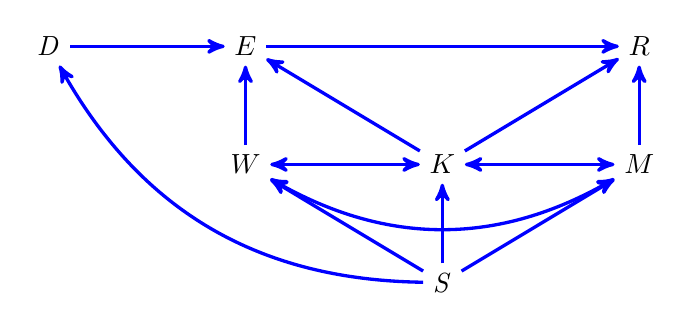
\begin{tikzpicture}[->,>=stealth']
    \tikzstyle{every state}=[draw=none]
    \node[] (D) at (0,0) {$\mathit{D}$};
    \node[] (AUC) at (2.5,0) {$E$};
    \node[] (WT) at (2.5,-1.5) {$W$};
    \node[] (EGFR) at (5,-1.5) {$K$};
    \node[] (CM) at (7.5,-1.5) {$M$};
    \node[] (S) at (5,-3) {$\mathit{S}$};
    \node[] (delta) at (7.5,0) {$R$};
    
      \path 
    	(D)  edge  [very thick, color=blue]    (AUC)  
    	(WT) edge  [very thick, color=blue]  (AUC)
    	(EGFR) edge  [very thick, color=blue]  (AUC)
      (AUC) edge  [very thick, color=blue]  (delta)
 
      (EGFR) edge  [very thick, color=blue]  (delta)
      (CM) edge  [very thick, color=blue]  (delta)

    	% (S) edge  [bend left=60, very thick, color=blue]  (E)
    	(S) edge  [very thick, color=blue]  (WT)
    	(S) edge  [very thick, color=blue]  (EGFR)
    	(S) edge  [very thick, color=blue]  (CM)
    	(S) edge  [very thick, color=blue, bend left]  (D)
    	
    	(WT) edge[<->, very thick, color=blue] (EGFR)
    	(CM) edge[<->, very thick, color=blue] (EGFR)
    	(WT) edge[<->, very thick, color=blue, bend right] (CM)
    	;
    \end{tikzpicture}
    \end{center}
    
        \caption{Abbreviated DINAMO selection diagram}
\end{figure}
    	
 
\begin{displaymath}
\begin{array}{rl}
D &= \mbox{dose or treatment status}  \\
E &= \mbox{exposure at PK steady-state}  \\
R &= \mbox{Change from baseline in hemoglobin A1c} \\
W &= \mbox{Body weight} \\
K &= \mbox{Kidney function (EGFR)} \\
M &= \mbox{Concomitant medication usage}
\end{array}
\end{displaymath}
 
 
 
 

 
\begin{displaymath}
\begin{array}{rlr}
\MoveEqLeft P^*(r \, | \, \mathrm{do}(d)) \\
&= \int_w \int_k \int_m  P^*(r \,|\, \mathrm{do}(d), w, k, m)  P^*(w, k, m \,|\, \mathrm{do}(d))\mathrm{d}m\mathrm{d}k \mathrm{d}w & \mbox{(Law of t.p.)} \\
&= \int_w \int_k \int_m \color{bark} P^*(r \,|\, \mathrm{do}(d), w, k, m) \color{pine} P^*(w, k, m) \color{black} \mathrm{d}m\mathrm{d}k \mathrm{d}w & ((W, K, M) \perp D)_{G_{\overline{D}}}
\end{array}
\end{displaymath} 



\begin{displaymath}
\begin{array}{rlr}
\color{bark}
&= \color{bark} \int_e P^*(r \,|\, \mathrm{do}(d), e, w, k, m) P^*(e  \,|\, w, k, m, \mathrm{do}(d)) \mathrm{d}e & \mbox{(Law of t.p.)} \\
&= \color{bark}  \int_e  P(r \,|\, \mathrm{do}(d), e, w, k, m)  P^*(e  \,|\, w, k, m, \mathrm{do}(d))  \mathrm{d}e &  \color{black} (R \perp S \,|\, W, K, M)_{G_{\overline{D}}} \\
&= \color{bark}  \int_e  P(r \,|\, \mathrm{do}(d), e, w, k, m)  P^*(e  \,|\, w, k, \mathrm{do}(d))  \mathrm{d}e &  \color{black} (E \perp M \,|\, W, K)_{G_{\overline{D}}} \\
% &= \color{bark}  \int_e  P(r \,|\, \mathrm{do}(d), \mathrm{do}(e), w, k, m)  P^*(e  \,|\, w, k, m, \mathrm{do}(d))  \mathrm{d}e &  \color{black} (R \perp E \,|\, W, K, M, D)_{G_{\overline{D}\underline{E}}} \\
&= \color{bark}  \int_e  \color {blueberry} P(r \,|\, e, k, m) \color{grapefruit} P^*(e  \,|\, w, k, \mathrm{do}(d)) \color{bark} \mathrm{d}e &  \color{black} (R \perp (W, D) \,|\, W, K, M, E)_{G_{\overline{D}}} \\
\end{array}
\end{displaymath} 

\begin{displaymath}
\begin{array}{rl}
 P^*(r \, | \, \mathrm{do}(d)) &=  \int_w \int_k \int_m \int_e \color{blueberry} P(r \,|\, e, k, m) \color{grapefruit} P^*(e  \,|\, w, k)  \color{pine} P^*(w, k, m) \color{black} \mathrm{d}m \mathrm{d}k \mathrm{d}w \mathrm{d}e  
\end{array}
\end{displaymath} 


 
%%%%%%%%%%%%%%%%%%%%
 
\begin{figure}[H]

\begin{center}
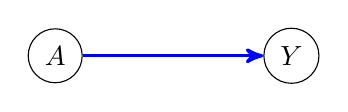
\begin{tikzpicture}[->,>=stealth']
\tikzstyle{every state}=[draw=none]
\node [shape=circle,draw](A) at (0,0) {$A$};
\node[shape=circle,draw] (Y) at (3,0) {$Y$};

  \path 

	(A)  edge [very thick, color=blue]  (Y)
	;
\end{tikzpicture}
\end{center}

 \caption{Simplest DAG}
\end{figure}




\begin{figure}[H]
\centering
\begin{subfigure}{.5\textwidth}
  \centering
  
  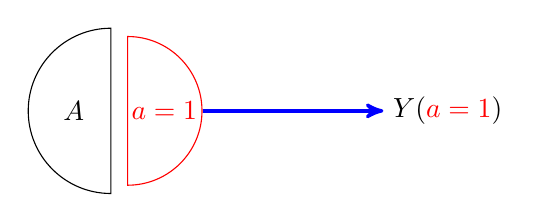
\begin{tikzpicture}[->,>=stealth']
\tikzstyle{every state}=[draw=none]
\node[shape=semicircle, draw, shape border rotate=90, inner sep=3.4mm] (A) at (0,0) {$A$};
\node[shape=semicircle, draw, shape border rotate=270, color=red, inner sep=0.5mm] (a) at (1.15,0) {$a=1$};
\node (Y) at (4.75,0) {$Y(\textcolor{red}{a=1})$};


  \path 
	(a)  edge  [very thick, color=blue]  (Y)
	;
\end{tikzpicture}

  \caption{SWIG for Experimental Treatment}
  \label{fig:sub1}
\end{subfigure}%
\begin{subfigure}{.5\textwidth}
  \centering

 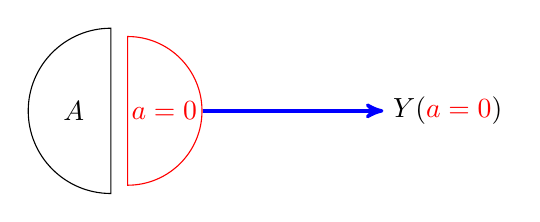
\begin{tikzpicture}[->,>=stealth']
\tikzstyle{every state}=[draw=none]
\node[shape=semicircle, draw, shape border rotate=90, inner sep=3.4mm] (A) at (0,0) {$A$};
\node[shape=semicircle, draw, shape border rotate=270, color=red, inner sep=0.5mm] (a) at (1.15,0) {$a=0$};
\node (Y) at (4.75,0) {$Y(\textcolor{red}{a=0})$};


  \path 
	(a)  edge  [very thick, color=blue]  (Y)
	;
\end{tikzpicture}

  \caption{SWIG for Reference Treatment}
  \label{fig:sub2}
\end{subfigure}
\caption{Two possible SWIGs for DAG in Figure 2}
\label{fig:test}
\end{figure}



\begin{figure}[H]
\centering

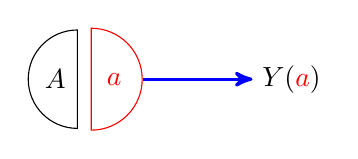
\begin{tikzpicture}[->,>=stealth']
\tikzstyle{every state}=[draw=none]
\node[shape=semicircle, draw, shape border rotate=90, inner sep=1.5mm] (A) at (0,0) {$A$};
\node[shape=semicircle, draw, shape border rotate=270, color=red, inner sep=2mm] (a) at (0.75,0) {$a$};
\node (Y) at (3,0) {$Y(\textcolor{red}{a})$};


  \path 
	(a)  edge  [very thick, color=blue]  (Y)
	;
\end{tikzpicture}
\caption{General graph representing the two SWIGs in Figure 3}
\end{figure}




\begin{figure}[H]
   
\begin{center}
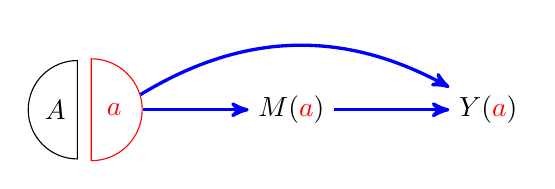
\begin{tikzpicture}[->,>=stealth']
\tikzstyle{every state}=[draw=none]
\node[shape=semicircle, draw, shape border rotate=90, inner sep=1.5mm] (A) at (0,0) {$A$};
\node[shape=semicircle, draw, shape border rotate=270, color=red, inner sep=2mm] (a) at (0.75,0) {$a$};
\node (M) at (3,0) {$M(\textcolor{red}{a})$};
\node (Y) at (5.5,0) {$Y(\textcolor{red}{a})$};

  \path 
	(a)  edge  [very thick, color=blue]                    (M)  
	(a)  edge  [bend left,very thick, color=blue]  (Y)
	(M)  edge  [very thick, color=blue]  (Y)						 
	;
\end{tikzpicture}
\end{center}
    
    \caption{SWIG for an ITT Estimand}
    
\end{figure}



\begin{align*}
 \Delta_{ITT} &= E[Y(1)] - E[Y(0)]  \\    
                            & = E[Y(1)|A=1]-E[Y(0)|A=0] \hspace{7.5mm} (Y(a) \independent A ) \\
                            & = E[Y|A=1]-E[Y|A=0] \hspace{18mm} (\text{consistency})   
\end{align*}




\begin{figure}[H]
    \begin{center}
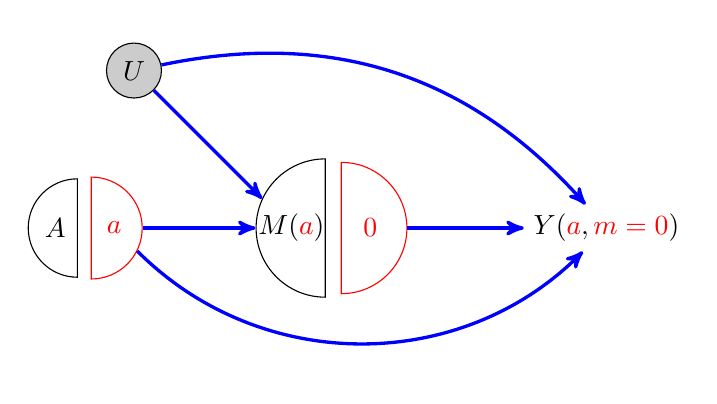
\begin{tikzpicture}[->,>=stealth']
\tikzstyle{every state}=[draw=none]

% Nodes
\node[shape=semicircle, draw, shape border rotate=90, inner sep=1.5mm] (A) at (0,0) {$A$};
\node[shape=semicircle, draw, shape border rotate=270, color=red, inner sep=2mm] (a) at (0.75,0) {$a$};

\node[shape=semicircle, draw, shape border rotate=90, inner sep=.1mm] (M) at (3,0) {$M(\textcolor{red}{a})$};
\node[shape=semicircle, draw, shape border rotate=270, color=red, inner sep=2.8mm] (m) at (4,0) {$0$};

\node (Y) at (7,0) {$Y(\textcolor{red}{a},\textcolor{red}{m=0})$};

\node[shape=circle,draw,fill=gray!40] (U) at (1,2) {$U$};

% Edges
  \path 
	(a)  edge  [very thick, color=blue]                    (M)  
	(a)  edge  [bend right,very thick, color=blue,out=-45,in=-135]  (Y)
	(m)  edge  [very thick, color=blue]  (Y)
	(U) edge    [very thick, color=blue]         (M)
	(U) edge    [bend left, very thick, color=blue]     (Y)							 
	;
\end{tikzpicture}
\end{center}
    \caption{SWIG for a hypothetical estimand with unobserved confounding}
    
\end{figure}



\begin{align*}
     \Delta_{hypo} &= E[Y(1,m)] - E[Y(0,m)]  \\    
                            & = E[Y(1,m)|A=1]-E[Y(0,m)|A=0] \hspace{7.5mm} (Y(a,m) \independent A ) 
\end{align*}



\begin{figure}[H]
\begin{center}
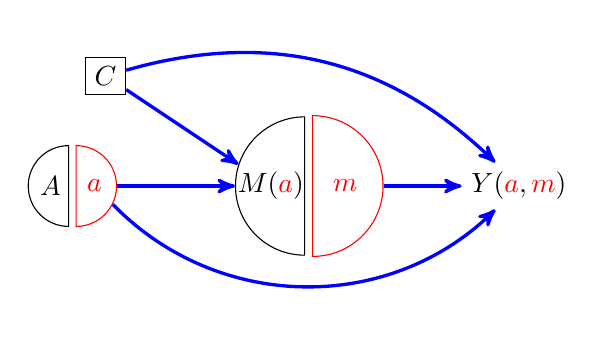
\begin{tikzpicture}[->,>=stealth',scale=0.7]
\tikzstyle{every state}=[draw=none]

% Nodes
\node[shape=semicircle, draw, shape border rotate=90, inner sep=1mm] (A) at (0,0) {$A$};
\node[shape=semicircle, draw, shape border rotate=270, color=red, inner sep=1.4mm] (a) at (0.8,0) {$a$};


\node[shape=semicircle, draw, shape border rotate=90, inner sep=.1mm] (M) at (4,0) {$M(\textcolor{red}{a})$};
\node[shape=semicircle, draw, shape border rotate=270, color=red, inner sep=2.6mm] (m) at (5.35,0) {$m$};

\node (Y) at (8.5,0) {$Y(\textcolor{red}{a},\textcolor{red}{m})$};
\node[shape=rectangle, draw] (C) at (1,2) {$C$};

  \path 
	(a)  edge  [very thick, color=blue]                    (M)  
	(a)  edge  [bend right,very thick, color=blue,out=-45,in=-135]  (Y)
	(m)  edge  [very thick, color=blue]  (Y)
	(C) edge    [very thick, color=blue]         (M)
	(C) edge    [bend left, very thick, color=blue]     (Y)							 
	;
\end{tikzpicture}
\end{center}
    \caption{SWIG for a hypothetical estimand with no unobserved confounding}
    
\end{figure}



\begin{figure}[H]
    
\begin{center}
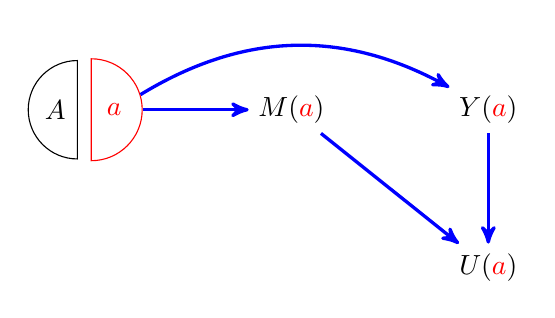
\begin{tikzpicture}[->,>=stealth']
\tikzstyle{every state}=[draw=none]
\node[shape=semicircle, draw, shape border rotate=90, inner sep=1.5mm] (A) at (0,0) {$A$};
\node[shape=semicircle, draw, shape border rotate=270, color=red, inner sep=2mm] (a) at (0.75,0) {$a$};
\node (M) at (3,0) {$M(\textcolor{red}{a})$};
\node (Y) at (5.5,0) {$Y(\textcolor{red}{a})$};
\node (U) at (5.5,-2) {$U(\textcolor{red}{a})$};

  \path 
	(a)  edge  [very thick, color=blue]                    (M)  
	(a)  edge  [bend left,very thick, color=blue]  (Y)	
        (M)  edge  [very thick, color=blue]  (U)						 
        (Y)  edge  [very thick, color=blue]  (U)
	;
\end{tikzpicture}
\end{center}
\caption{SWIG for a composite estimand}
    
\end{figure}



\begin{figure}[H]
\begin{center}
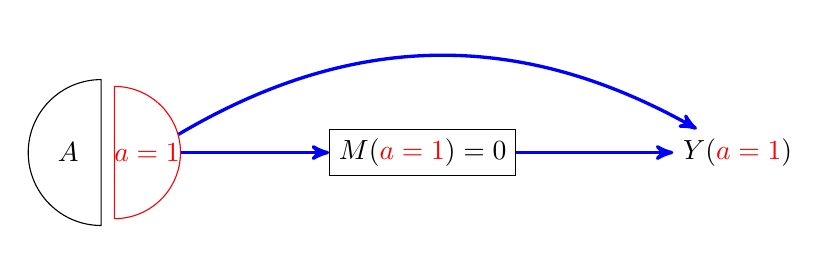
\begin{tikzpicture}[->,>=stealth']
\tikzstyle{every state}=[draw=none]
\node[shape=semicircle, draw, shape border rotate=90, inner sep=2.85mm] (A) at (0,0) {$A$};
\node[shape=semicircle, draw, shape border rotate=270, color=red, inner sep=.01mm] (a) at (1,0) {$a=1$};
\node[shape=rectangle, draw] (M) at (4.5,0) {$M(\textcolor{red}{a=1})=0$};
\node (Y) at (8.5,0) {$Y(\textcolor{red}{a=1})$};

  \path 
	(a)  edge  [very thick, color=blue]                    (M)  
	(a)  edge  [bend left,very thick, color=blue]  (Y)
	(M)  edge  [very thick, color=blue]  (Y)						 
	;
\end{tikzpicture}
\end{center}
\caption{SWIG where active treatment is given for those who would not have the IE under treatment (i.e. conditioning on $M(a=1)=0$)}
\end{figure}


\begin{figure}[H]
\begin{center}
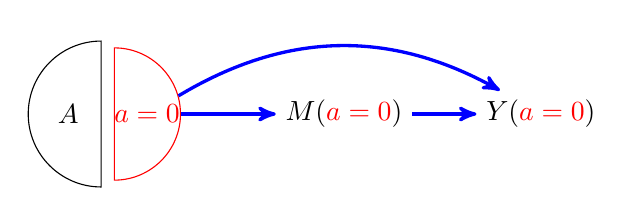
\begin{tikzpicture}[->,>=stealth']
\tikzstyle{every state}=[draw=none]
\node[shape=semicircle, draw, shape border rotate=90, inner sep=2.85mm] (A) at (0,0) {$A$};
\node[shape=semicircle, draw, shape border rotate=270, color=red, inner sep=.01mm] (a) at (1,0) {$a=0$};
\node (M) at (3.5,0) {$M(\textcolor{red}{a=0})$};
\node (Y) at (6,0) {$Y(\textcolor{red}{a=0})$};

  \path 
	(a)  edge  [very thick, color=blue]                    (M)  
	(a)  edge  [bend left,very thick, color=blue]  (Y)
	(M)  edge  [very thick, color=blue]  (Y)						 
	;
\end{tikzpicture}
\end{center}
\caption{SWIG where reference treatment is given for those who would not have the IE under treatment $M(a=1)=0$}
\end{figure}





\begin{itemize}
    \item $M_1$ = Intake of short acting pain relief medication
    \item $M_2$ = Treatment discontinuation due to Adverse Event, Loss of Efficacy, or intake of prohibited medications
    \item $M_3$ = Change of dose of allowed concomitant medication for pain
    \item $M_4$ =  Treatment discontinuation due to Administrative or Other reasons
\end{itemize}


\begin{figure}[H]
\begin{center}
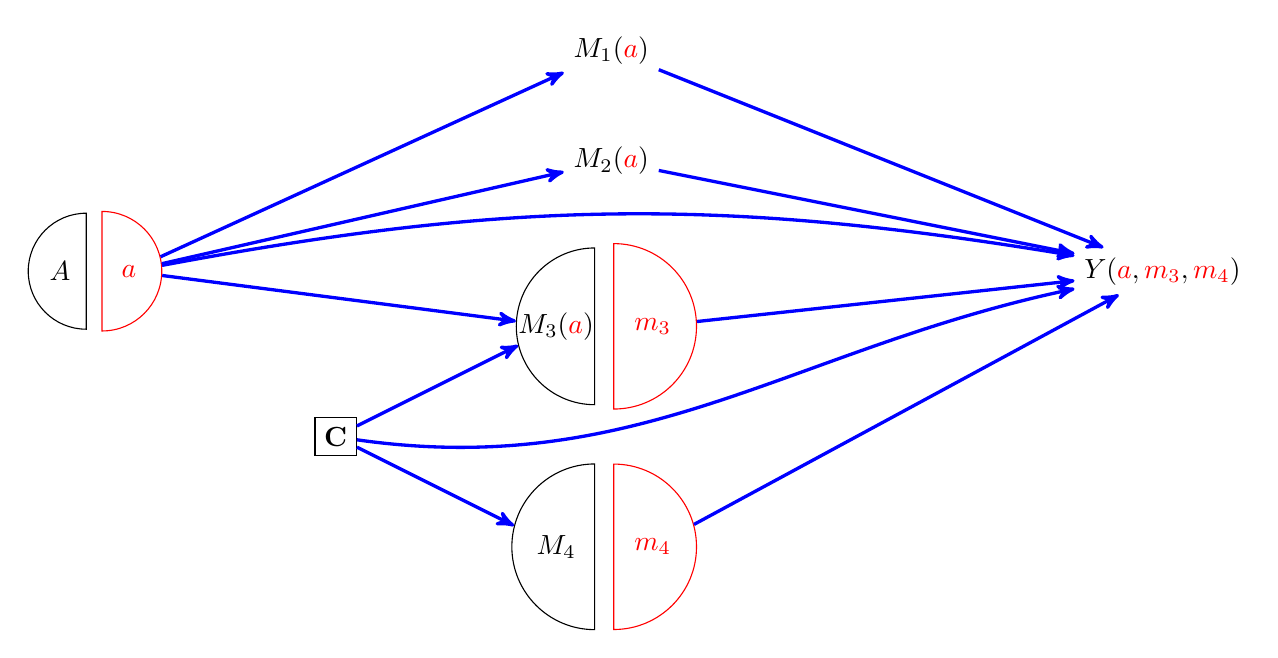
\begin{tikzpicture}[->,>=stealth',scale=0.7]
\tikzstyle{every state}=[draw=none]

%%%%%%%% Nodes %%%%%%%%

% Treatment
\node[shape=semicircle, draw, shape border rotate=90, inner sep=2mm] (A) at (0,0) {$A$};
\node[shape=semicircle, draw, shape border rotate=270, color=red, inner sep=2.5mm] (a) at (1.25,0) {$a$};

% IE
\node (M1) at (10,4) {$M_1(\textcolor{red}{a})$};
\node (M2) at (10,2) {$M_2(\textcolor{red}{a})$};

\node[shape=semicircle, draw, shape border rotate=90, inner sep=.1mm] (M3) at (9,-1) {$M_3(\textcolor{red}{a})$};
\node[shape=semicircle, draw, shape border rotate=270, color=red, inner sep=2.6mm] (m3) at (10.75,-1) {$m_3$};

\node[shape=semicircle, draw, shape border rotate=90, inner sep=2.4mm] (M4) at (9,-5) {$M_4$};
\node[shape=semicircle, draw, shape border rotate=270, color=red, inner sep=2.6mm] (m4) at (10.75,-5) {$m_4$};

\node (Y) at (20,0) {$Y(\textcolor{red}{a},\textcolor{red}{m_3},\textcolor{red}{m_4})$};

\node[shape=rectangle, draw] (C) at (5,-3) {$\textbf{C}$};

  \path 
	(a)  edge  [very thick, color=blue]                    (M1)  
	(a)  edge  [very thick, color=blue]                    (M2)  
	(a)  edge  [bend left,very thick, color=blue,out=10,in=170]  (Y)
	(a)  edge  [very thick, color=blue]                    (M3)  
	
	
	(M1)  edge  [very thick, color=blue]                    (Y)  
	(M2)  edge  [very thick, color=blue]                    (Y)  
	(m3)  edge  [very thick, color=blue]                    (Y)
	(m4)  edge  [very thick, color=blue]                    (Y)
	
	
	
	%(m)  edge  [very thick, color=blue]  (Y)
	(C) edge    [very thick, color=blue]         (M3)
	(C) edge    [very thick, color=blue]         (M4)
	(C) edge    [bend right, very thick, color=blue,out=-20,in=180]     (Y)							 
	;
\end{tikzpicture}
\end{center}
    \caption{SWIG for a Clinical Trial in Chronic Pain}
    
\end{figure}






\end{document}
